\documentclass[12pt]{article}

\usepackage{amsmath}
\usepackage{graphicx}
\usepackage[numbers]{natbib}
\usepackage{titling}
\usepackage{float}
\usepackage[hidelinks]{hyperref}
\usepackage{amsthm}

\graphicspath{{assets/}}
\bibliographystyle{IEEEtranN}

\newcommand{\wideimage}[2][]{%
  \makebox[\textwidth][c]{\includegraphics[width=1.2\textwidth,#1]{#2}}%
}

\pretitle{%
  \vspace*{-5cm}
  \begin{center}
  
\includegraphics[width=\textwidth]{uniLogo.png}\\
  \vspace*{3cm}
}
\posttitle{\end{center}}

\title
{
    {\Huge Creating and Optimising a Fluid Simulation using Smoothed Particle Hydrodynamics} \\
    \vspace*{1cm}
    {\LARGE BSc Computer Science}
}

\author
{
    \vspace*{0.1cm}\huge Sakir Azimkar \\
    \vspace*{1cm}\huge 200823588 \\
    \large Supervised by: Richard Davison
}

\date{April 2025}

\begin{document}
    \maketitle
    \newpage
    \pagenumbering{arabic}

    \section*{Abstract}
    This dissertation explores the Navier-Stokes equations, which are used to describe the motion of fluids. It briefly looks at an Eulerian implementation introduced by Jos Stam\cite{stam}, before shifting focus on to Lagrangian methods - specifically Smoothed Particle Hydrodynamics (SPH). Furthermore, this paper describes an implementation of this technique. \\ The main goal of this project is to produce a real-time fluid simulation that can be integrated into a video game, with minimal performance loss. It is an optimisation problem, motivated by an interest in the GPU and shader languages. The final project is a Smoothed Particle Hydrodynamics simulation that can reach 400 frames per second with over thirty-two thousand particles on modern hardware.
    
    \newpage

    \section*{Declaration} ``I declare that this dissertation represents my own work, unless explicitly stated otherwise."

    \newpage

    \section*{Acknowledgements}
    I would like to express my deepest gratitude to my supervisor, Richard Davison, for being reliable and helpful throughout the entire project. I'd also like to thank Gary Ushaw, my ``second" supervisor, who was always encouraging and present at our meetings. Lastly, I'd like to thank my friends and family for supporting me during this time. This dissertation is dedicated to these people.
    
    \newpage
    \tableofcontents
    \newpage
    \listoffigures
    \newpage

    \section{Introduction}
    This section highlights the motivations, aims and objectives of this project. It talks about the overall dissertation structure and compares the differences between this project and the initial proposal.
    
    \subsection{Motivation}
    Fluid dynamics are observed in all aspects of daily life and in research. It is crucial to be able to simulate and understand the behaviour of all fluids, including liquids and gases. There already exists a number of different techniques to achieve this, through utilisation of the Navier-Stokes equations. These methods have been crucial in research and in industry. For example in aerospace, which utilises Computational Fluid Dynamics (CFD) for aerodynamic analysis, aircraft design optimisation and thermal management, to name just a few. As our knowledge of fluids and CFD techniques improve, the global market is expected to increase by nearly triple its current value by 2033\cite{market}. Simulations are also essential for cost reduction, as they reduce the need for physical prototypes, which are significantly more expensive to produce.

    In the gaming industry, realistic fluid dynamics are essential to enhance immersion; being able to interact with the ocean in a beach environment is a lot more engaging than the common use of invisible barriers that prevent interaction with the water in many games. A fantastic example of excellent water physics is \textit{Far Cry 6}\cite{farcry6}, as it looks very realistic and is affected by external forces from objects such as vehicles and people swimming.
    
    However, affordable options for advanced fluid simulation are quite difficult to come by for indie developers, who do not have the same funding as triple A companies like \textit{Ubisoft}. As a result, the motivation for this project is to produce a free, lightweight simulation for all types of fluid (not just water). It will also aim to maintain a high performance, so it may be seamlessly implemented into an existing video game with minimal performance loss. This is essential in the gaming industry as lag and low frame rates hinder the overall gameplay experience.

    \subsection{Aim}
    The aim of this dissertation is to utilise the Navier-Stokes equations and Smoothed Particle Hydrodynamics to produce an accurate fluid simulation. The performance (specifically frame rate) of the simulation will be measured and there will be attempts to optimise it. The resulting code should be a 3D fluid flow video game asset that works for Unity.

    \subsection{Objectives}
    \begin{enumerate}
        \item \textbf{Explore Existing Fluid Simulations} - This dissertation will test and experiment with free and accessible simulations available on the internet. It will compare and identify issues with them from the perspective of a game developer searching for a tool to implement into their own game.
        \item \textbf{Navier-Stokes and SPH} - This dissertation will explain what the Navier-Stokes equations are and describe two ways to utilise them in a fluid simulation.
        \item \textbf{OpenGL and C++/GLFW} - This dissertation will briefly mention a graphics API that was used initially in this project and explain why it was chosen. It will then talk about the issues experienced with this API and why it was not utilised in the final project.
        \item \textbf{Unity and Compute Shaders} - This dissertation will talk about the use of Unity and compute shaders to produce a fluid simulation that runs on the GPU.
        \item \textbf{Frame Rate and Performance Investigations} - Throughout this dissertation, the main focus will be on improving the frame rate of the simulation. It will talk about what methods were used to improve the frame rate, such as reprogramming the simulation in shader languages. The overall goal will be to improve the performance of the simulation.
    \end{enumerate}

    \subsection{Changes}
    In the initial project proposal, it was stated that the simulation would be programmed in \textit{C++}, using \textit{GLFW}\cite{glfw} to create windows and display the graphics created by the graphics API that I would be using, \textit{OpenGL}\cite{opengl}. However, later in development this decision was changed to utilising the \textit{Unity} game engine\cite{unity} and compute shaders. Reasoning will be provided in the What was Done and How section.

    Additionally, the project proposal stated that the simulation would be first created in two dimensions and later upgraded to three. It was decided to skip this step as the development process was mostly the same, the only difference being whether the vectors contained two or three values. This was to save development time and allow more focus on optimisation.

    \subsection{Dissertation Structure}
    
    \subsubsection{Time Structure}
    
    \begin{figure}[H]
        \makebox[\textwidth][c]{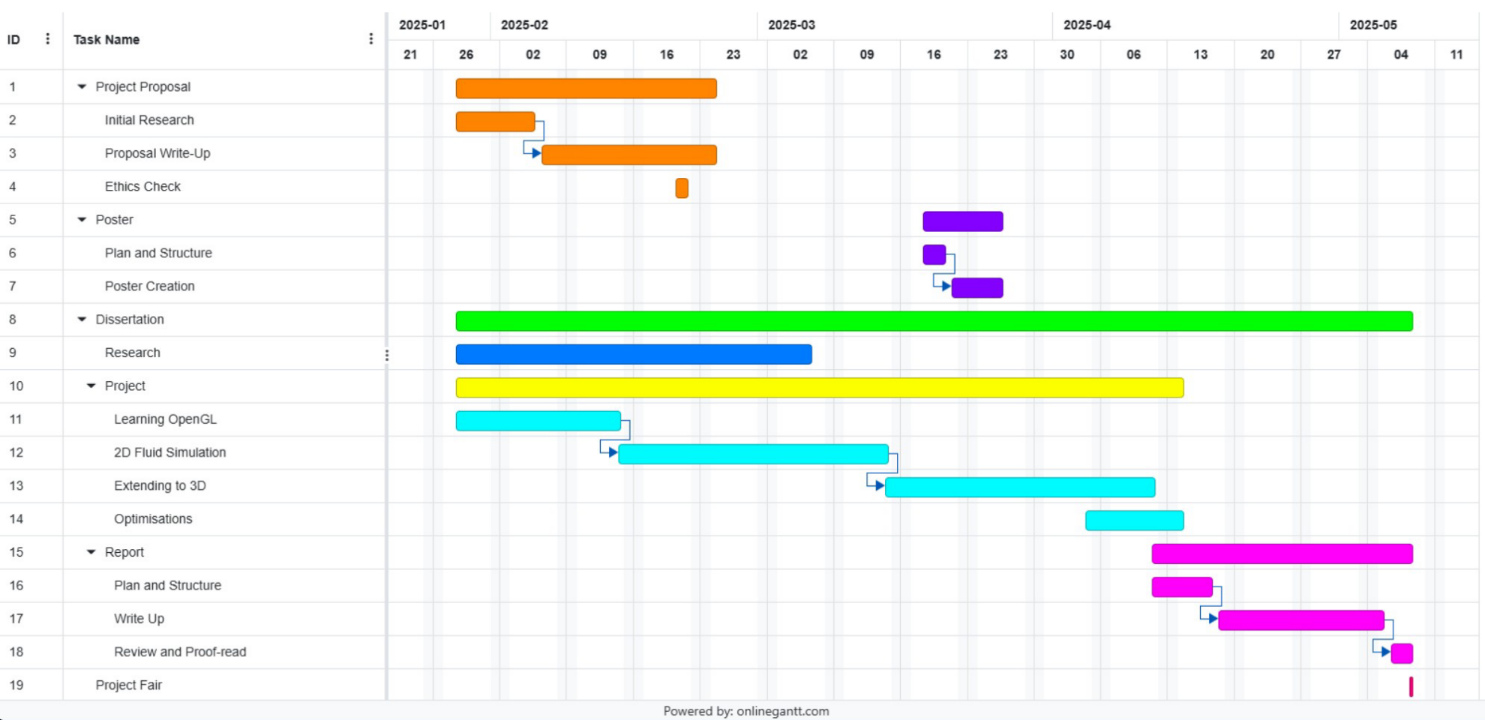
\includegraphics[width=1.4\textwidth]{ganttChart.png}}%
        \caption{Gantt chart of project timeline \cite{onlinegantt}}
    \end{figure}

    \subsubsection{Dissertation Outline}

    \begin{itemize}
        \item \textbf{Introduction} \\
        An introduction to the dissertation, outlining the motivation, aim, objectives and overall project structure. 
        \begin{itemize}
            \item Motivation
            \item Aim
            \item Objectives
            \item Changes
            \item Structure
        \end{itemize}
        \item \textbf{Background Review} \\
        A breakdown of research performed before and during the project.
        \begin{itemize}
            \item Existing fluid simulations
            \item Software Tools
        \end{itemize}
        \item \textbf{What was Done and How} \\
        An explanation of how the simulation was implemented, including the methods learned and processes involved.
        \begin{itemize}
            \item Mathematics and Physics
            \item OpenGL
            \item Unity
            \item Compute Shaders
            \item GPU Instancing
            \item Optimisations
        \end{itemize}
        \item \textbf{Results and Evaluation} \\
        A complete analysis of frame rate improvements over the course of the project and results obtained.
        \begin{itemize}
            \item Frame Rate
            \item Testing
        \end{itemize}
        \item \textbf{Conclusion} \\
        A conclusion that describes fulfilment of objectives, what was learned and future work.
        \begin{itemize}
            \item Aims and Objectives
            \item Achievements
            \item What was Learned
            \item Future Work
        \end{itemize}
    \end{itemize}

    \section{Background Review}
    This section shows the research made on this dissertation. It talks about relevant background resources that were used for different parts of the development process.
    
    \subsection{Strategy}
    There are three main components that needed to be researched at the start of this project:
    \begin{itemize}
        \item Exploring existing fluid simulations
        \item Software Tools
        \item Fluid simulation methods
    \end{itemize}
    \sloppy
    All three of these sections are integral in achieving a functional, lightweight simulation and thus needed to be researched before beginning. Below is an outline of the papers, videos and other resources that were used to understand these topics.

    \subsection{Exploring existing fluid simulations}
    It is important to understand current existing options that are available and describe their benefits and limitations in the context of video games.

    \subsubsection{WebGL Implementations}

    ``WebGL (Web Graphics Library) is a JavaScript API for rendering interactive 2D and 3D graphics within any compatible web browser without the use of plug-ins. WebGL is fully integrated with other web standards, allowing GPU-accelerated usage of physics, image processing, and effects in the HTML canvas".\cite{webglwikipedia}

    There are a lot of fantastic \textit{WebGL} implementations of fluid motion that are easily accessible due to their availability in a web browser. An example is the one developed by PavelDoGreat on GitHub.

    \begin{figure}[H]
        \noindent\wideimage[]{webGLGas.png}
        \caption{\textit{WebGL} Fluid Simulation by PavelDoGreat on GitHub \cite{webgl1}}
    \end{figure}

    This simulation showcases a gaseous fluid made up of different, randomly-generated colours. They appear to mostly be for aesthetic purposes. The screen begins completely black and requires the user to input an external force by left-clicking and moving the cursor across the screen. There is a control panel on the top right corner, which allows the user to change various settings, such as density diffusion and vorticity. This is a great visual aid for educational purposes as it allows the user to see the visual impacts that these variables have on the fluid in real time. As an educational tool, this is an excellent visual aid; the immediate feedback and colorful representation make it easy to understand complex fluid dynamics concepts. In the context of video games, however, the colours are a bit unnecessary. This can be easily rectified if someone were to use it in their game, but they would need to make a number of modifications to the existing code to make it independent of user input (for the more common uses of fluids in games).

    Here is another example of a \textit{WebGL}-based fluid simulation available for free online, developed by Grant Kot.

    \begin{figure}[H]
        \noindent\wideimage[]{webGLParticles.png}
        \caption{\textit{WebGL} Fluid Simulation by Grant Kot. \cite{webgl2}}
    \end{figure}
    
    This simulation excels in visualising fluid interactions, particularly between liquids of varying masses - represented by four distinct colors. You can use the mouse and different keybinds to manipulate the fluid with a range of forces, such as lifting a portion of it up (as shown in figure 3), or creating dynamic collision objects that follow the cursor. It behaves with realistic motion that is driven by gravity and internal pressure and user interaction is only optional.

    Conversely, there is a performance issue with this project. During testing, the simulation peaked at around fifty frames per second. This is completely fine when exploring the fluid in a web browser or for educational demos, but becomes a much larger issue when using it as a video game asset, as video games prefer to be consistently above 60 frames per second - to maintain responsiveness and overall gameplay fluidity. Further optimisations would be required of this simulation in order to utilise it in a video game environment.

    WebGL simulations, however, work exceptionally in very simple browser games. Here is an example called \textit{Interplanetary Postal Service}\cite{ips}, which was created by Sebastian Macke, for a coding competition with a strict 13KB size limit.

    \begin{figure}[H]
        \noindent\wideimage[]{webGLIPS.png}
        \caption{\textit{Interplanetary Postal Service} by Sebastian Macke \cite{ips}}
    \end{figure}

    As the game's core mechanics are very simple (use WASD to power the post lander on to the landing pads), there is very little need for optimisations. This allows it to run consistently at over 60 frames per second. This demonstrates how WebGL-based simulations can deliver high performance and smooth interactivity when used for lightweight, focused experiences - which most video games aren't.

    While all of these examples are incredibly impressive, they would not function well in more complicated, non-web-based video games. The first two are built as standalone browser-based visualisations for the purposes of aesthetics and education. Although all of these can be rewritten and ported to OpenGL-based games, there is a lot of upfront work required to do so; they do not work out-of-the-box. They are also only two-dimensional, which means further modifications would be required necessary to adapt them for 3D environments. Furthermore, for games written using pre-existing game engines such as Unity, most of the existing JavaScript simulation code would have to be rewritten into a language that is compatible with the engine, such as \textit{C\#}. One of the aims of this dissertation is to produce a 3D asset that is ready to use in Unity without requiring extensive modifications.

    \subsubsection{Unity Assets}

    There are a few choices on the \textit{Unity Asset Store}\cite{unityasset}. However, there are a few issues with each of the available options.

    \begin{figure}[H]
        \noindent\wideimage[]{obiFluid.png}
        \caption{\textit{Obi Fluid}, Unity Asset \cite{obi}}
    \end{figure}

    The most popular option appears to be \textit{Obi Fluid}, which advertises ``multi-threaded AAA quality fluid simulations" on its store page. From the screenshots and videos provided, this does appear to be the case. However, with its steep price tag, it is difficult to verify as many developers are understandably hesistant to spend over £40 on a single asset. Additionally, the store page mentions that the simulation may have performance issues in larger projects and should only be used for smaller scale projects or 2D game simulations, making it an unfit choice for 3D games or large bodies of fluid.

    \begin{figure}[H]
        \noindent\wideimage[]{KWS.png}
        \caption{\textit{KWS Water System Standard} \cite{kws}}
    \end{figure}

    Another fantastic asset is the \textit{KWS Water System}. It has a lot of incredibly useful features, such as refraction, volumetric lighting and screen space reflections. Furthermore, it has optimisations implemented such as instanced rendering and view culling, so it is possible to simulate much larger bodies of fluid with minimal performance issues. This would be an outstanding asset for video games, if it weren't for the even steeper price tag of over £60.

    In addition to these examples, there are many available assets that don't simulate actual fluid motion or behavior, but instead create the illusion of it by only simulating the surface. This is a suitable option for games that don't require fluid interaction, but that falls outside the scope of this dissertation. One of the main motivations of this project is that the simulation is accessible to all kinds of developers, so it will be free unlike these examples.
    
    \subsubsection{Fluids in Video Games}

    It is also important to understand the fluid simulations that are actively present in existing video games. There aren't many games allow the player to interact with the water physically, due to the high performance cost required to implement these features.

    \begin{figure}[H]
        \noindent\wideimage[]{fromDust.png}
        \caption{\textit{From Dust} Gameplay \cite{fromdustvideo}}
    \end{figure}

    \textit{From Dust}\cite{fromdust} is a god game where the player manipulates matter such as lava, soil and water. In the gameplay video\cite{fromdustvideo}, it is clear that the sand when placed and moved around displaces the water realistically. While the visual quality of the static sea surface may appear simplistic by modern standards, the game's real-time manipulation of large quantities of matter was groundbreaking for its era over thirteen years ago. Albeit impressive visually, there was a lot of computational resources required to run such a large scale simulation. As a result, there was quite a few complaints about the game being capped at thirty frames per second\cite{dsog}, which was very low even back then.
    
    \begin{figure}[H]
        \noindent\wideimage[]{clairObscur.png}
        \caption{A screenshot of water blocked by an invisible wall in Clair Obscur: Expedition 33}
    \end{figure}

    Even nowadays there are a lot of video games that don't utilise realistic fluid flows because of their high computational resource requirement. An example of this is with a game that released just this month, \textit{Clair Obscur: Expedition 33}\cite{clairobscur}.
    While the simulation is visually stunning, it is not possible to interact with the water. There is a loss of immersion here, especially considering the position of this water. It is located at the end of the prologue, after the character has left the island they have resided on their entire life to explore the abandoned mainland. The character, having never before set foot beyond their home, should be experiencing a profound sense of unfamiliarity due to a heavy environment change. The static and artificial appearance of the river diminishes this intended narrative impact, disconnecting the character from the player.

    \begin{figure}[H]
        \noindent\wideimage[]{farCry6.png}
        \caption{Helicopter physics in Far Cry 6 \cite{farcry6video}}
    \end{figure}

    A modern game that does an excellent job at fluid simulation is \textit{Far Cry 6}. As shown in Figure 9, the wind produced by the helicopter's turbines visibly pushes the water away from the vehicle. Furthermore, the player is able to swim and dive into the fluid, as well as observe external forces acting upon it when objects, such as explosives, are thrown into the water. This would be an ideal fluid simulation approach for many games seeking realistic water interactions. However there are a few issues with this. Since \textit{Far Cry 6} is a proprietary, AAA game, its source code is not visible to the public, as thus the simulation is not accessible by anyone else.
    
    Since the release of this game, the former water lead tech, Zhenyu Mao, has moved on to other projects with \textit{Lightspeed Studios}, and has developed a new water rendering solution for games. In an interview\cite{zhenyu}, Mao mentions ``Thanks to Dr. Wu's expertise, we have developed a proprietary solution that generates natural water flow that interacts harmoniously with the environment. Our water simulation can generate accurate flow around objects, creating realistic turbulence and generating foam in the appropriate places." This sounds incredibly promising, but is currently still a proprietary, in-house solutiona available to \textit{Lightspeed Studios} only. There is a presentation available online about the physics behind this solution\cite{zhenyupresent}, but that is not in the scope of this dissertation.

    \subsubsection{Conclusion}

    While there are a lot of fluid simulations available online, few are practical for use within 3D video games; they are often computationally taxing and thus would not be a feasible asset to utilise without significant prior optimisation and modifications. The options that do satisfy these conditions are usually proprietary and restricted to the studio it was developed in - or come at a premium cost inaccessible to some developers. Therefore, the motivation for this dissertation is to develop a freely accessible, efficient 3D fluid simulation that can be integrated into modern video games without significant performance trade-offs.

    \subsection{Software Tools}

    Choosing the correct set of tools is essential for an optimisation problem. They must be lightweight in nature and avoid unnecessary overhead in order to achieve the best performance possible.

    \subsubsection{Graphics API vs. Existing Game Engine}

    \begin{figure}[H]
        \noindent\wideimage[]{unityInterface.png}
        \caption{Empty Unity\cite{unity} scene}
    \end{figure}

    Game engines have the advantage of simplicity, leading to a faster development cycle. There are a lot of available pre-built tools, editors and assets that allow rapid prototyping and game development. For the purposes of this dissertation, many of these tools are not necessary. For instance, the physics engine will not be utilised as all physics will be manually coded. However, many of these tools would be beneficial for this project. For example, all linear algebra calculations related to camera depth and appearance have already been implemented. This means that by simply loading a model into the scene, it will automatically be rendered in 3D with realistic lighting. This saves the hassle of writing it all from scratch if a grpahics API were to be implemented.

    Game engines also benefit from large, active communities. There are plenty of tutorials, forums and online resources created by other developers. This makes it easier to find solutions to common problems, whether they involve problem solving or bug fixing. Graphics APIs are not as commonly utilised due to their increased complexity and thus have fewer resources available. However, there are two great tutorials for both \textit{OpenGL} and \textit{Vulkan}\cite{vulkan} that fully explain and provide an implementation for the setup of the graphics rendering pipeline \cite{learnopengl}\cite{vulkantutorial}.

    Graphics APIs have the added benefit of greater control and customisation due to their lack of abstration and increased level of understanding required. Every phase in the graphics rendering pipeline can be controlled manually, giving the developer more freedom and flexibility. There is also no overhead from the game engine, which may also slightly improve performance. Furthermore, once a project is begun within an engine, it is bound by its licenses, giving the developer less freedom.

    Due to an enthusiasm to learn more about the graphics rendering pipeline and more low-level graphics interactions, it was decided at this point that a graphics API would be utilised over a game engine. Aforementioned in the project proposal, this was with the caveat that a swap to a game engine (specifically \textit{Unity}, due to prior experience) would occur if insufficient progress was made in the strict timeframe of this project. Considering the changes made to this dissertation in comparison to the project proposal, it is clear that this alteration was eventually realised.

    \subsubsection{OpenGL vs. Vulkan}

    As a graphics API was decided, the next choice was between \textit{OpenGL} and \textit{Vulkan}. \textit{DirectX} was not considered due to its lack of cross-platform compatability, as it was specifically designed for \textit{Windows} and \textit{XBox}. This was a relatively simple decision, as \textit{OpenGL} is considered the beginner option, and \textit{Vulkan} is not recommended for new graphics programmers by Alexander Overvoorde, the writer of \textit{Vulkan Tutorial}: ``Vulkan is targeted at experienced graphics programmers. You should start with an easier language than C++ and an easier API than Vulkan'' \cite{vulkancomment}. Although \textit{Vulkan} is a better choice for future-proofing (as \textit{OpenGL} is no longer receiving updates), this reasoning was not significant justification due to the ability to rewrite this project with more experience and time. Thus, \textit{OpenGL} was selected, accompanied by the C++ language due to previous experience with the language.
    
    \subsection{Fluid Simulation methods}

    This section talks about two simulation methods involving the Navier-Stokes equations.

    \subsubsection{Navier-Stokes Equations}

    \begin{equation}
        \frac{\partial{\textbf{u}}}{\partial{t}} + (\textbf{u} \cdot\nabla)\textbf{u} = v\nabla^2 \textbf{u} - \frac{1}{\rho}\nabla p + \textbf{f}
    \end{equation}

    Equation 1 is a non-linear partial differential equation that describes fluid motion\cite{slides}. The first term, $\frac{\partial{\textbf{u}}}{\partial{t}}$, represents the change in velocity over time at a fixed point, where $\textbf{u}$ is the velocity field of the fluid. $-(\textbf{u}\cdot\nabla)\textbf{u}$ is called the advection term. Advection is described as ``the transport of a substance or of heat by the flow of a liquid"\cite{cambridge}. In fluid dynamics, this may also refer to the transport of a property due to fluid flow. $\nabla$ is a vector of partial derivatives: $\nabla = (\frac{\partial}{\partial x}, \frac{\partial}{\partial y}, \frac{\partial}{\partial z})$. Taking the dot product of \textbf{u}, a vector, and this operator, $\textbf{u}\cdot\nabla$, gives us a directional derivative - it describes the direction that a property is changing.

    \begin{equation*}
        (\textbf{u}\cdot\nabla)\textbf{u} \equiv u_x \frac{\partial \textbf{u}}{\partial x} + u_y \frac{\partial \textbf{u}}{\partial y} + u_z \frac{\partial \textbf{u}}{\partial z}
    \end{equation*}

    This term thus describes the advection of velocity, which is also referred to as convective acceleration, ``the effect of acceleration of a flow with respect to space''\cite{nswikipedia}.

    There are three more terms on the right hand side of the equation: the diffusion/viscosity term, pressure and external forces. Sometimes written as $\nabla \cdot (v\nabla\textbf{u})$, the viscosity term describes how the fluid motion is damped due to its viscosity. Fluids with a higher viscosity constant $v$ tend to have stronger resistance, resulting in stronger smoothing and slower flows. $\nabla^2$ is also known as the Laplacian operator. The Laplacian is obtained by summing the second partial derivative with respect to each variable component-wise:

    \begin{equation*}
        \nabla^2\textbf{u} \equiv (\frac{\partial^2{u_x}}{\partial{x^2}} + \frac{\partial^2{u_x}}{\partial{y^2}} + \frac{\partial^2{u_x}}{\partial{z^2}}, \frac{\partial^2{u_y}}{\partial{x^2}} + \frac{\partial^2{u_y}}{\partial{y^2}} + \frac{\partial^2{u_y}}{\partial{z^2}}, \frac{\partial^2{u_z}}{\partial{x^2}} + \frac{\partial^2{u_z}}{\partial{y^2}} + \frac{\partial^2{u_z}}{\partial{z^2}})
    \end{equation*}

    Multiplying this value by a viscosity constant determines how much the velocity is smoothed or evened-out by viscous forces. If the Laplacian is positive, it means that the velocity is lower at that point than its neighbours, so a larger positive force is applied; a negative Laplacian applies force in the opposite direction.

    Pressure is simply defined as ``the amount of force acting on a certain area"\cite{bbcbitesize}, or force acting per unit area. As a result, a pressure gradient produces a force that pushes the fluid from areas of high pressure to areas of low pressure. This is described by the second term, $-\frac{1}{\rho}\nabla{p}$, where $\nabla{p}$ is the pressure gradient, and $\rho$ is the density of the fluid at this position. Since gradients point in the increasing direction, the negative is taken so the fluid moves away from the direction of increasing pressure. Additionally, this gradient value gives force acting per unit volume, but the previous terms have been accelerations. This is corrected using Newton's Second Law, $F = ma$. Since density is the mass per unit volume of the fluid, the pressure gradient is multiplied by the reciprocal of the density to obtain the acceleration. Below is a correction of the SI units to obtain acceleration.

    \begin{proof}
        $$\left[\nabla{p}\right] = \frac{N}{m^3} = \frac{kg \cdot ms^{-2}}{m^3} = \frac{kg}{m^2\cdot s^2}$$
        $$\left[\rho\right] = \frac{kg}{m^3}$$
        $$\frac{\left[\nabla{p}\right]}{\left[\rho\right]} = \frac{kg}{m^2 \cdot s^2} \cdot \frac{m^3}{kg} = \frac{m}{s^2}$$
    \end{proof}
    
    The final term accounts for external forces that act on the fluid, such as gravity. These forces are included to correctly describe changes in momentum according to Newton's Second Law.

    \begin{equation}
        \frac{\partial{\rho}}{\partial{t}} = -(\textbf{u}\cdot\nabla)\rho + \kappa\nabla^2 \rho + S
    \end{equation}

    Equation 2 has very similar structure to Equation 1, however this one is used in the calculation of a scalar quantity, density. As a result, there is no pressure force term, and external forces is replaced by an external source term S, which adds or removes density from the system. The viscosity constant is also replaced with $\kappa$, the diffusion constant. This measures how fast the property (in this case density) diffuses through the fluid.

    \subsubsection{Eulerian Implementations}

    Eulerian, or grid-based implementations for fluid dynamics treat the fluid as a grid of cells.
    
    \begin{figure}[H]
        \begin{center}
            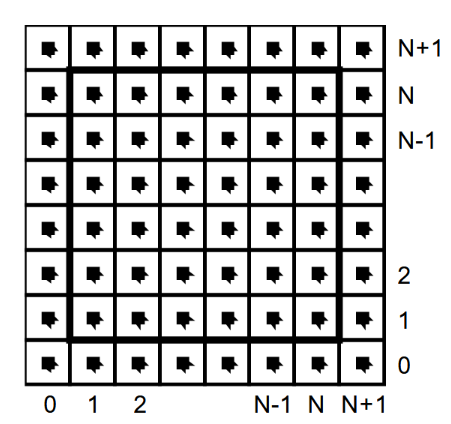
\includegraphics{gridFluid.png}
        \end{center}
        \caption{Computational grid with densities and velocities defined in their centres \cite{stam}}   
    \end{figure}

    Figure 11 is a computation grid of cells by Jos Stam. There is an extra layer of cells around the grid to account for boundary conditions. This method utilises Equation 2 to produce a density diffusion solver, where each cell either adds or removes density from its neighbours. Due to distance of other cells, there is no need to include any others in this calculation, as their impact will be negligible and slow the simulation down quite considerably.

    \begin{figure}[H]
        \begin{center}
            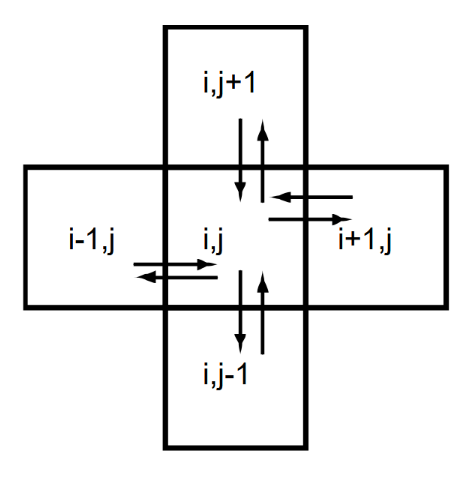
\includegraphics{neighbourDiff.png}
        \end{center}
        \caption{Density exchange through diffusion between neighbours \cite{stam}}   
    \end{figure}

    After this diffusion has occured, the centres of the grids are considered as particles and are traced through the velocity field, calculated with Equation 1. In order to convert the ``particles" back into grid cells, there are two grids used: a grid of cells containing the old density values and a second grid containing the new density values. The new positions are traced backwards through the velocity field to find the original grid cell, and assign this value to the new position.

    There are a lot of different ways to achieve fluid flow with Eulerian implementations and this is a very oversimplified description, but the main premise of this method is to utilise grids and the two equations mentioned.

    \begin{figure}[H]
        \begin{center}
            \noindent\wideimage[width=0.7\textwidth]{eulerianEG.png}
        \end{center}
        \caption{Eulerian simulation \cite{eulerianeg}}
    \end{figure}

    \subsubsection{Lagrangian Implementations}

    Langrangian implementations of fluid flow involve treating the fluid as small parcels or particles of fluid. These particles influence their neighbours but are not confined to grid cells. As a result, more calculations are required in determining which particles are within influenceable range. A classic example of a Lagrangian method is Smoothed Particle Hydrodynamics (SPH).

    SPH was initially developed by Gingold, Monaghan and Lucy in 1977 for the pusposes of astrophysics\cite{sca}. Since the particles are independent nodes, this method is meshfree, which improves its implementation and parallelisation. Considering the expensive computations required, parallelisation is fundamental in improving performance for the simulation. Furthermore, conservation of mass is guaranteed; the particles represent mass and the particles do not disappear at any stage.

    Furthermore, this method simplifies the Navier-Stokes equations the following generalised SPH equation:

    \begin{equation}
        A_S(\textbf{r}) = \sum_{j}{m_j \frac{A_j}{\rho_j}W(\textbf{r} - \textbf{r}_j, h)}
    \end{equation}

    For each particle with location $\textbf{r}$, we iterate through every other particle $j$ with mass $m_j$, density $\rho_j$, position $\textbf{r}_j$ and property $A_j$ to calculate that particle's total property quantity. $W$ is a smoothing kernel that is defined differently for each property. After a large enough distance $\lvert\textbf{r} - \textbf{r}_j\rvert$, also referred to as the smoothing radius, the value of the smoothing kernel becomes 0; the particle is too far away to provide any significant influence. As a result, this calculation only needs to be performed on particles that are close enough, a key optimisation step for this method.

    \section{What Was Done and How}

    \subsection{Learn OpenGL}


    \section{Results and Evaluation}
    \subsection{Results}
    \subsection{Evaluation}

    \section{Conclusion}
    \subsection{Aims and Objectives}
    \subsection{What Was Learned}
    \subsection{Future Work}

    \newpage
    \section{References}
    \bibliography{references}

    \newpage
    \section{Appendices}

    \subsection{Unity Asset Store}

    \begin{figure}[H]
        \noindent\wideimage[]{unityStore1.png}
        \caption{Most popular results for "fluid simulation" \cite{unityasset}}
    \end{figure}

    \begin{figure}[H]
        \noindent\wideimage[]{unityStore2.png}
        \caption{Cheapest results for "fluid simulation" \cite{unityasset}}
    \end{figure}

    \begin{figure}[H]
        \noindent\wideimage[]{stylizedWaterURP.png}
        \caption{Example of surface-only Unity asset \cite{stylized}}
    \end{figure}


\end{document}